\chapter{Introduction}
% Introduction section
%  1. Introduction.
%  2. Background and setting. 
%  3. Identification of problem
%  4. Purpose Statement. 
%  5. Objectives or research questions
%  6. Assumptions. Limitations. Definition of terms
%  7. Significance of the study.

% Introduction section (from unsw.edu.au)
% Move A: establish your territory (say what the topic is about)
%   1.  state the general topic and give some background
%   2.  provide a review of the literature related to the topic
%   3.  define the terms and scope of the topic
Optimization plays an important part in our everyday life, science development, product design, and
much more. Examples of optimization could be choosing the optimal way to commute from A to B,
deciding what songs should land on your playlist, or constructing the strongest possible bridge using
limited material. In general, optimization is the art of choosing the best decision among a set of possible
decisions. Often we try to quantify how good a decision is: A bus takes 20 min, a car takes 15 min to go from A to B, How would
you rate the song? This bridge construction costs 10 million kroner. If it is possible to come up with a
quantification of how good a decision is in terms of a real number, then we can define the optimization problem as
\textit{mathematical} optimization problem: 
$$\min_{x\in \mathcal{X}} f(x)$$ where the functional $f: \mathcal{X} \rightarrow \mathbb{R}$ is
called the objective function and $\mathcal{X}$ is the set of possible decisions (or decisions you
consider). Note that the optimization problem is formulated as a minimization problem. If one identifies
the optimal decision as a maximum of $f$ (instead of the minima), then finding the minima in the
negating the objective function $-f(x)$ is equivalent. Throughout this thesis, we refer to
optimization as minimizing the objective function. The optimization problem is now in the domain of 
numbers and here many algorithms have been developed to find the minimum of the function
$f(\cdot)$.

Evaluation of the objective function can be cheap (e.g. if it just requires summing/multiplying
numbers) or highly expensive (e.g. if it involves human rating, large simulation, or physical
experiments). In the latter case, we want to avoid evaluating the objective function as much as
possible - we want to use \textit{sample efficient} optimization. The overall topic of this
thesis, \textit{Bayesian optimization}, is one of the preferred frameworks for sample efficient optimization. 

Bayesian optimization is a probabilistic surrogate-based optimization methodology: Assuming some samples from a
highly expensive objective, then a cheap (surrogate) function is used to fit the samples. The next sample
is found by minimizing the surrogate and the process is repeated. Bayesian optimization seeks to
enhance this procedure with probability theory, where the surrogate function becomes a probabilistic (Bayesian)
regression model. The most common choice is a Gaussian Process, as it encapsulates the uncertainty very well,
but also because its inference procedure (computing answers to probability queries like $p(y|x)$) is exact.

% Move B: establish a niche (show why there needs to be further research on your topic)
%   4.  outline the current situation
%   5.  evaluate the current situation (advantages/ disadvantages) and identify the gap

Even though GP has proven good for many cases, there will be problems where its assumptions do not
hold. E.g the commonly seen GP with an isotropic kernel (covariance between two points is invariant to
translation in input), yields a strong assumption about the continuity of the objective function and that
the objective function behaves similarly throughout the domain $\mathcal{X}$. In Figure
\ref{fig:GP_vs_BNN} we see an example of how the GP's uncertainty quantification is going wild due
to a discontinuity in the underlying objective function (a small varying step-function). In some areas is it very common to have
these discontinuities, for instance, in material discovery where it is well known that materials often
change very suddenly \cite{Nature_BO_paper}. To accommodate these challenges the literature introduces more
flexible kernel functions for the GP, however, this introduces additional hyperparameters and since
we often only deal with a small amount of data, tuning and computation can be significantly challenging \cite{Nature_BO_paper}.

\begin{figure}[H]%
    \centering
    {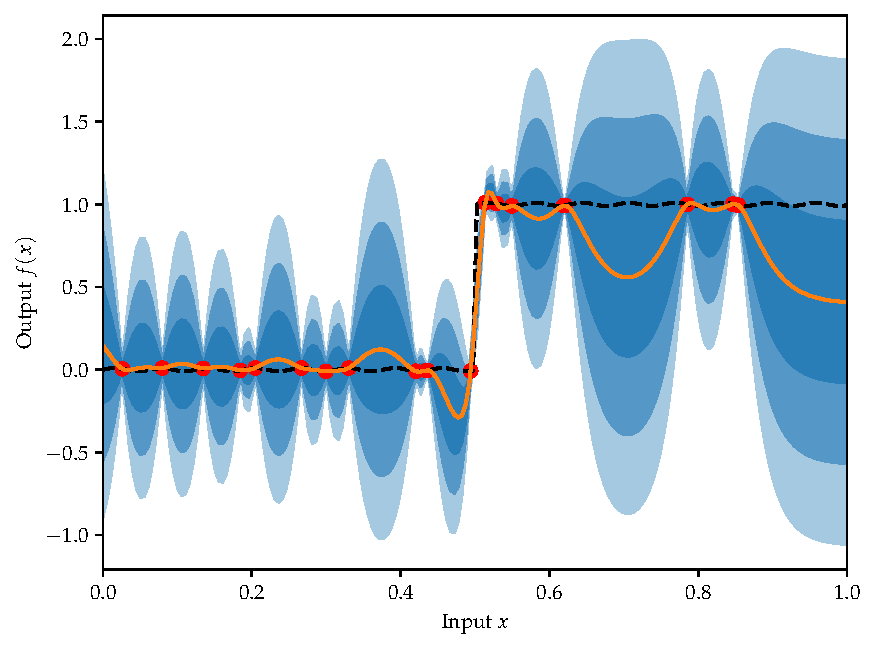
\includegraphics[width=0.46\textwidth]{Pictures/GP_vs_BNN1.pdf} }%
    \qquad
   {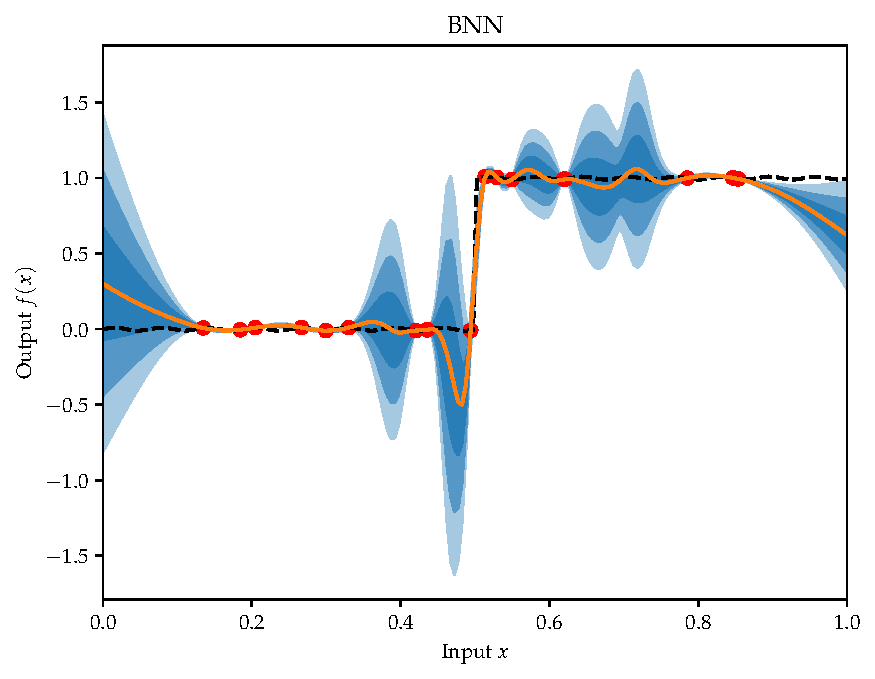
\includegraphics[width=0.46\textwidth]{Pictures/GP_vs_BNN2.pdf} }%
    \caption{Left: GP fitted to 20 data points. Right: A Bayesian neural network fitted to the same points.
    The objective function is the dashed black line. This examplifies how a discontinuerity makes the 
    standard implemented GP (optimized with emperical bayes) overreact to all other areas in the domain $[0,1]$,
    while the Bayesian NN only express uncertainty where the discontinuerity happen $x = 0.5$}%
    \label{fig:GP_vs_BNN}
\end{figure}


% Move C: introduce the current research (make hypotheses; state the research questions)
%   6.  identify the importance of the proposed research
%   7.  state the research problem/ questions
%   8.  state the research aims and/or research objectives
%   9.  state the hypotheses
%   10. outline the order of information in the thesis
%   11. outline the methodology

GPs are very attractive models since they allow for exact inference, a closed-form expected improvement (more on this later)
 and in general good uncertainty quantification.
However, as we saw in the figure \ref{fig:GP_vs_BNN} maybe we can do better! 
If it is possible to sample a few times less from the objective function, it can potentially
save hours of work, lots of money, or energy (Depending on what is demanded to evaluate the objective
function). It is therefore relevant to investigate if other models will perform better. As
mentioned, the assumptions of GP can be too strong. In this thesis, we aim to create models with less strong
assumptions, which can perform better on certain types of (complex) problems, and just as well as the GP on most types of  
problems. 

\section{Contribution}
This thesis investigates surrogate models alternative to GP, more concretely Bayesian NN
and mixture regression. The proposed hypotheses are,
\begin{enumerate}
    \item Neural Networks perform better applied to complex BO problems than GPs.
    \item Mixture regression models like SPN can be employed as an effective surrogate model
    performing better than GPs and Neural Networks in some complex cases. 
\end{enumerate}

Note what is meant by performance is \textit{sample efficiency}, i.e. how few evaluations of the objective function
are necessary to find the minima. So even though the surrogate modeling and optimization can be really slow, 
it is assumed that the objective function is very expensive, so a slow surrogate model would not matter.

% 1) Firstly, we want to examine what types of problems a GP surrogate is not a good choice and
% where Bayesian neural nets (BNN) surrogates can have an advantage (inspiration found in this 2020
% thesis \cite{PhDthesis})
    
% 2) Looking at sum product networks (SPN) as novel surrogate models. A SPN is - similarly to a BNN
% - a deep probabilistic model and still expressive but with tractable inference, which potentially
% could lead to advantages over BNNs. 

\section{Related work}
Here we give a short overview of research in different surrogates for Bayesian optimization
and the very related field active learning. The different surrogate models, which are in the 
research we found, 
\begin{itemize}
    \item Gaussian Process
    \item Bayesian neural network
    \item Random forest
    \item Kernel estimator
    \item Bayesian multivariate adaptive regression splines (BMARS)
    \item Bayesian additive regression trees (BART)
\end{itemize}

Often the main focus has been on lowering the computational complexity of inference while
showing performance is (or almost is) as well as GPs. Inference time of the GP scales cubic with the
number of data points and only linear for Bayesian Neural Network. Lowering the inference time is also the
main focus of the Ph.D. thesis "Sample-efficient Optimization Using Neural Networks" from 2020
\cite{PhDthesis}, but chapter 3 showcases empirically that using Bayesian neural networks as
surrogate models performed better, or at least comparable to GPs on a wide number of
problems. The performance difference was more clear for high-dimensional problems. 
<mention BOHAMIANN and DNGO>

The 2021 nature paper "Bayesian optimization with adaptive surrogate models for automated experimental design"
\cite{Nature_BO_paper}, focus on the sample efficiency of the BO applied to autonomous materials discovery, 
which yields a relatively high-dimensional design space and non-smooth patterns of objective functions.  
The paper shows that using Bayesian multivariate adaptive regression splines
and Bayesian additive regression trees as alternative surrogate models outperform GP significantly, 
for complex BO problems. 

Active learning is closely related to Bayesian Optimization, but here the focus is on learning the underlying function
using as few samples as possible instead of just finding its minima. 
In active learning, a Gaussian process is also very common, but the paper "Active Learning with Statistical Models" \cite{ALStatisticalModels}
investigates using Gaussian mixtures and kernel estimitor in active learning, i.e. as a surrogate model for selecting
the next samples. These are regression models not seen much in the literature, which
is modeling the joint distribution of x and y, and using the conditional distribution $p(y|x)$
as the regression model. The results were ... ??

\section{Structure of the thesis}
The structure of the thesis is
\begin{itemize}
    \item The first chapter introduces the concept of optimization in general, Bayesian optimization 
    and how surrogates/Bayesian regression models are relevant.
    \item The second chapter introduces GP and Bayesian Neural Networks
    \item The third chapter introduces the mixture regression and the novel new SPN regression.
    \item The fourth chapter results
    \item Finally a discussion and conclusion.
\end{itemize}
% Introduction to Optimization, and Bayesian optimization. 
% Presentation of different surrogate models. 
% Experiments using the different surrogates. 



% \section{No free lunch and surrogate reseach}

% <No free lunch theorem for optimization>, establish some questions on why there is no best method.
% And a burning research problem is if it is possible to use a different surrogate model than the GP. 
% And whether or not they in general performs better? What assumptions underlie the problem. 
% The assumption for GP regression is that the objective function follows a Gaussian process, whereas
% we assume it follows a random forest or neural network. These are assumptions that yields, consideration:
% Is this a good assumption? Bayesian NNs are very expressive. 

%   10. outline the order of information in the thesis
%   11. outline the methodology


% \section{Old intro}
% %<What is optimization>
% Optimization plays an important part in our everyday life, science development, and product design.
% What different transportation should you choose to get fast from A to B, what songs should
% land on your playlist, and what is the optimal bridge construction. Mathematical optimization problems 
% are all problems in the form, 
% $$\min_{x\in \mathcal{X}} f(x)$$ where $f: \mathcal{X} \rightarrow \mathcal{R}$ is a functional. I.e
% if it is possible to set up an objective function. e.g. what is the cost of the bridge given a
% specific design, or how pleasant you think some music, and some constraints such that you keep in
% the domain of interest. Evaluation of the objective function can be cheap e.g. if it just requires
% summing and multiplying numbers or highly expensive if it involves human rating or large simulation
% and physical experiments. Bayesian optimization is a preferred <ref> framework for optimization of
% the expensive objective functions. And is also referred to as \textit{sample efficient}
% optimization. 
% %<Why Bayesian optimization?>

% Bayesian optimization is a probabilistic surrogate-based optimization: Assuming some samples from a
% highly expensive objective a cheap (surrogate) function is used to fit the samples. The next sample
% is found by minimizing the surrogate and the process is repeated. Bayesian optimization seeks to
% enhance this procedure with probability theory, where the surrogate function becomes a probabilistic
% regression model. The most common choice is a Gaussian Process, as it encapsulates the uncertainty very well,
% but also because its inference procedure (computing answers to probability queries like $p(y|x)$) is exact.

% Even though GP has proven good for many cases, there will be problems where the assumptions do not hold. 
% The assumptions of a GP are essential that the objective function can be described as a GP.
% The nature of a GP is highly dependent on the choice of its kernel and the parameters chosen in that kernel. 
% Another reason for the popularity of the GP is the closed-form inference and giving a closed-form of the 
% expected improvement aqurisition function. 

% The PhD thesis "Sample-efficient Optimization Using Neural Networks" from 2020 \cite{PhDthesis}
% showcases empirically that using Bayesian neural networks as surrogate models performed better,
% or at least comparable to GPs on a wide number of problems. The performance difference was more
% clear for high-dimensional problems. 

% This master thesis project will investigate surrogate models alternative to Gaussian processes in
% Bayesian optimization. Firstly by examining what types of problems a GP surrogate is not a good
% choice for and where Bayesian neural nets (BNN) surrogates can have an advantage (inspiration found in
% this 2020 thesis [1]). Secondly by looking at sum-product networks (SPN) as novel surrogate models.
% An SPN is - similarly to a BNN - a deep probabilistic model and still expressive but with tractable
% inference, which potentially could lead to advantages over BNNs. 

% %#<Short overview of types of surrogate models>

% <Make a figure of how the parts are all connected>

\section{notation}
Throughout this thesis we will be using Bayesian notation, i.e. $p(x) := P(X=x)$ is the probability
density function of the random variable $X$ evaluated in $x$. and $p(y|x) := P(Y=y|X=x)$ or $p(y|x)
:= P(Y|X=x)$. And writing $p(y^2|x)$ means $P(Y^2=y^2|X=x)$ and \textbf{not} $P(Y=y^2|X=x)$

The density of a normal distribution evaluated in $x$ is denoted as, $\mathcal{N}(x|\mu, \Sigma)$. 

We will not distinguish between vectors and scalars notation-wise unless it is not clear from the 
context. 

% \section{related work}
% This thesis is 
% <BAHAMIANN>

% <DNGO>
% Focus on the inference time of GP scales cubic, which is not appropriate for
% parallel BayesOpt. 
% Experiments on 6dim Hartmann function. 

% <Arayns paper.>
% Conclusions..!?

% Already developed alternative surrogate models has been found in the litterateur. The last presented
% surrogate model, SPN, is to our knowledge not in any published work. More models might still be
% added to the list. 

% \subsubsection*{DNGO}
% Deep Networks for Global Optimization (DNGO) is presented in the paper 2015 paper "Scalable Bayesian
% Optimization Using Deep Neural Networks"\cite{snoek2015scalable}. The surrogate model is a neural
% network, where only the last layer is probabilistic, this leads to Bayesian regression and very fast
% inference.  

% \subsubsection*{BOHAMIANN}
% \textbf{B}ayesian \textbf{O}ptimization with \textbf{Hami}ltonian Monte Carlo \textbf{A}rtificial
% \textbf{N}eural \textbf{N}etworks (BOHAMIANN) is presented in the 2016 paper "Bayesian Optimization
% with Robust Bayesian Neural Networks"\cite{NIPS2016_a96d3afe}. This is a fully Bayesian Neural
% Network trained using adaptive Hamiltonian MCMC. 